\begin{figure}
  \centering
  \begin{subfigure}[b]{\linewidth}
    \centering
    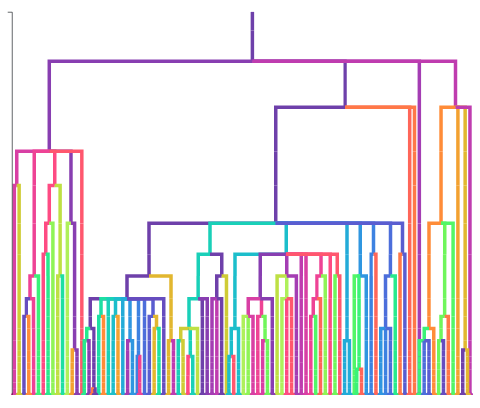
\includegraphics[width=\textwidth, height=0.16\textheight]{img/plain_resolution_3}
    \caption{33\% resolution}
    \label{fig:plain-perfect-and-reconstruction-phylogenies:resolution_3}
  \end{subfigure}
  \begin{subfigure}[b]{\linewidth}
    \centering
    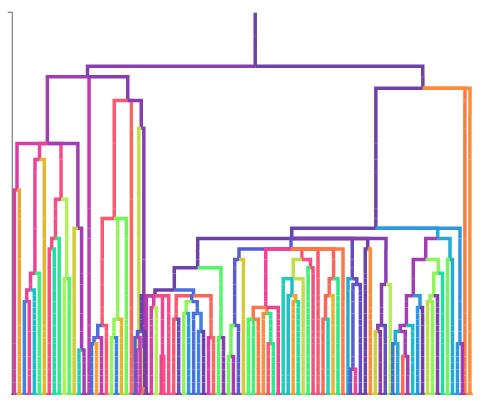
\includegraphics[width=\textwidth, height=0.16\textheight]{img/plain_resolution_10}
    \caption{10\% resolution}
    \label{fig:plain-perfect-and-reconstruction-phylogenies:resolution_10}
  \end{subfigure}
  \begin{subfigure}[b]{\linewidth}
    \centering
    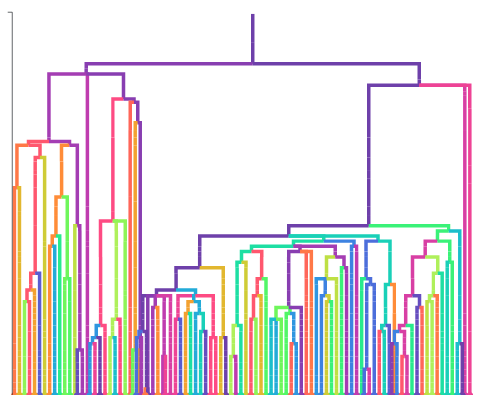
\includegraphics[width=\textwidth, height=0.16\textheight]{img/plain_resolution_30}
    \caption{3\% resolution}
    \label{fig:plain-perfect-and-reconstruction-phylogenies:resolution_30}
  \end{subfigure}
  \begin{subfigure}[b]{\linewidth}
    \centering
    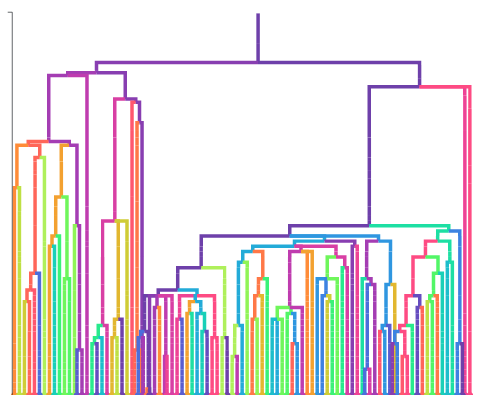
\includegraphics[width=\textwidth, height=0.16\textheight]{img/plain_resolution_100}
    \caption{1\% resolution}
    \label{fig:plain-perfect-and-reconstruction-phylogenies:resolution_100}
  \end{subfigure}
  \begin{subfigure}[b]{\linewidth}
    \centering
    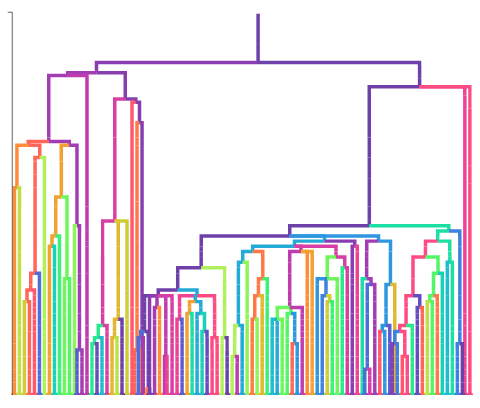
\includegraphics[width=\textwidth, height=0.16\textheight]{img/reference}
    \caption{reference tree}
    \label{fig:plain-perfect-and-reconstruction-phylogenies:reference}
  \end{subfigure}
  \caption{Comparison of phylogeny reconstructions using our agglomerative trie-based algorithm using different hereditary stratigraphy resolutions. For the purposes of visualization, these trees contain a sub-sample of 100 leaf nodes out of the 32,000 in the full trees. Sub-figures are arranged from top to bottom in increasing order of resolution.}
  \label{fig:plain-perfect-and-reconstruction-phylogenies}
\end{figure}
